Consider the one-dimensional, transient (i.e. time-dependent) 
heat conduction equation without heat generating sources
\begin{equation}
\rho C_p \frac{\partial T}{\partial t} 
= \frac{\partial }{\partial x} \left(  k  \frac{\partial T}{\partial x} \right)
\end{equation}
where $\rho$ is density, $C_p$ heat capacity, $k$ thermal conductivity, $T$ temperature, 
$x$ distance, and $t$ time. 

If the thermal conductivity, density and heat capacity are constant over the model domain, 
the equation can be simplified to a diffusion equation:
\begin{equation}
\frac{\partial T}{\partial t} =  \kappa \frac{\partial^2 T}{\partial x^2} 
\end{equation}
where $\kappa=k/\rho C_p$ is the heat diffusivity. \index{general}{Heat Diffusivity}

We wish to solve this PDE in time and space (provided the appropriate 
boundary conditions have been given). The domain is $[0,L_x]$
and it is discretised by means of $nnx$ points as depicted hereunder:

\begin{center}
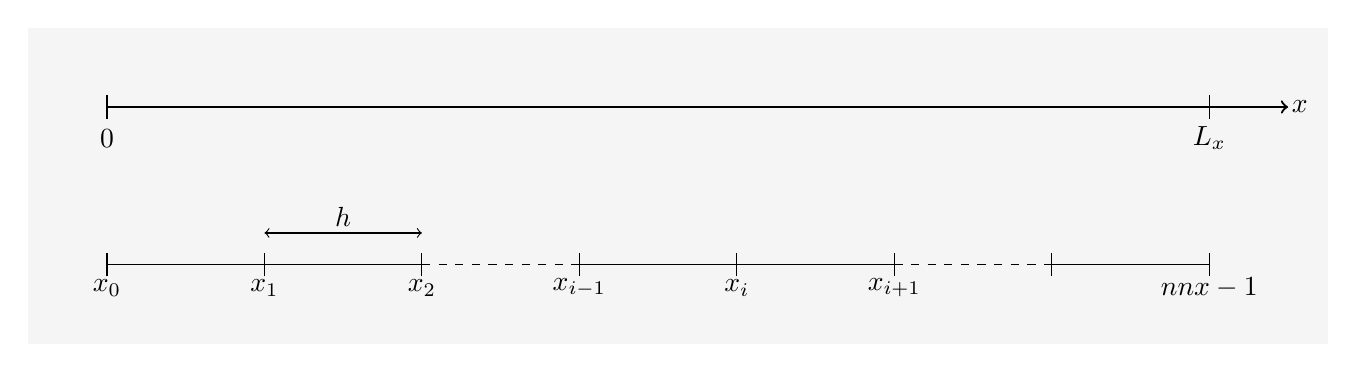
\begin{tikzpicture}
\draw[fill=gray!8,gray!8](0,0) rectangle (16.5,4);
%\draw[step=0.5cm,gray,very thin] (0,0) grid (16.5,4); %background grid
\node[] at (16.15,3) {$x$};
\node[] at (1,2.6) {$0$};
\node[] at (15,2.6) {$L_x$};
\draw[-] (1,2.85) -- (1,3.15) ; 
\draw[-] (15,2.85) -- (15,3.15) ; 
\draw[thick,->] (1,3) -- (16,3) ; 

%\draw[fill=gray!13,gray!13](1,1) rectangle (8,3);
%\draw[thick] (1,1) -- (5,1) -- (5,4) -- (1,4) -- cycle;  

\draw[-] (1,1) -- (5,1) ; 
\draw[dashed] (5,1) -- (7,1) ; 
\draw[-] (7,1) -- (11,1) ; 
\draw[dashed] (11,1) -- (13,1) ; 
\draw[-] (13,1) -- (15,1) ; 

\draw[-] (1,0.85) -- (1,1.15) ; 
\draw[-] (3,0.85) -- (3,1.15) ; 
\draw[-] (5,0.85) -- (5,1.15) ; 
\draw[-] (7,0.85) -- (7,1.15) ; 
\draw[-] (9,0.85) -- (9,1.15) ; 
\draw[-] (11,0.85) -- (11,1.15) ; 
\draw[-] (13,0.85) -- (13,1.15) ; 
\draw[-] (15,0.85) -- (15,1.15) ; 

\node[] at (7,0.7) {$x_{i-1}$};
\node[] at (9,0.7) {$x_i$};
\node[] at (11,0.7) {$x_{i+1}$};

\node[] at (1,0.7) {$x_0$};
\node[] at (3,0.7) {$x_1$};
\node[] at (5,0.7) {$x_2$};
\node[] at (15,0.7) {$nnx-1$};

\draw[<->] (3,1.4) -- (5,1.4) ; 
\node[] at (4,1.6) {$h$};

\end{tikzpicture}


\end{center}

The derivative of temperature with regards to time can be approximated
with a forward finite difference approximation {\it in time} as
\begin{equation}
\frac{\partial T}{\partial t} 
\simeq \frac{T_{i}^{n+1}-T_i^n}{t^{n+1}-t^n} 
= \frac{T_{i}^{n+1}-T_i^n}{\delta t} 
\end{equation}
where $\delta t$ is the time step, i.e. the time between two consecutive 
measurements (the equivalent of $h$ in space). 
In all that follows the subscript will always refer to space indices 
while the superscript will always refer to time indices.
To be clear: $n$ represents the current time step whereas $n+1$
represents the next time step. 

Both $n$ and $i$ are integers; $n$ varies from 0 to $nstep-1$ (total number of time steps)
and $i$ varies from 0 to $nnx-1$ (where $nnx$ is the total number of grid points in $x$-direction).

The spatial derivative is replaced by a central FD approximation
\begin{eqnarray}
\frac{\partial^2 T}{\partial x^2} 
\simeq \frac{T_{i+1}^n - 2T_i^n + T_{i-1}^n}{h^2}
\end{eqnarray}
We obtain
\begin{eqnarray}
\frac{T_{i}^{n+1}-T_i^n}{\delta t} 
= \kappa \frac{T_{i+1}^n - 2T_i^n + T_{i-1}^n}{h^2}
\end{eqnarray}
and finally
\begin{eqnarray}
\boxed{
T_i^{n+1}=T_i^n + \delta t \; \kappa \frac{T_{i+1}^n - 2T_i^n + T_{i-1}^n}{h^2}
}
\end{eqnarray}

Because the temperature at the current time step $n$ is known,
we can compute the new temperature without solving any additional equations.
Such a scheme is an {\bf explicit} finite difference method and
was made possible by the choice to evaluate the temporal derivative with forward differences.

\begin{center}


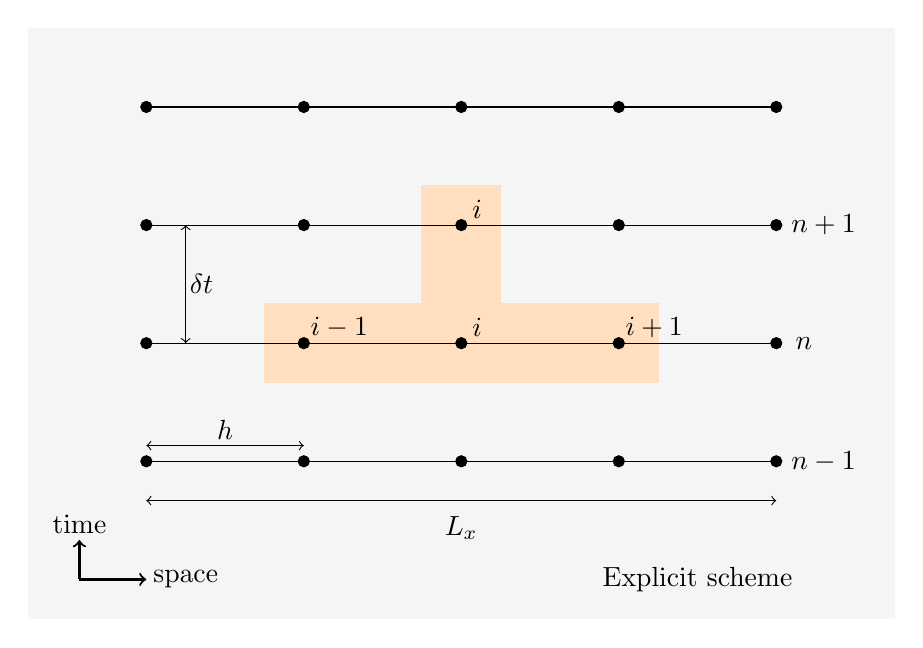
\begin{tikzpicture}
\draw[fill=gray!8,gray!8](-0.5,0) rectangle (10.5,7.5);


\draw[fill=orange,orange!25](2.5,3) rectangle (7.5,4);
\draw[fill=orange,orange!25](4.5,4) rectangle (5.5,5.5);
%\draw[step=0.5cm,gray,very thin] (0,0) grid (10.5,7.5); %background grid

\draw[black,fill=black] (1,2)  circle (2pt);
\draw[black,fill=black] (3,2)  circle (2pt);
\draw[black,fill=black] (5,2)  circle (2pt);
\draw[black,fill=black] (7,2)  circle (2pt);
\draw[black,fill=black] (9,2)  circle (2pt);

\draw[black,fill=black] (1,3.5)  circle (2pt);
\draw[black,fill=black] (3,3.5)  circle (2pt);
\draw[black,fill=black] (5,3.5)  circle (2pt);
\draw[black,fill=black] (7,3.5)  circle (2pt);
\draw[black,fill=black] (9,3.5)  circle (2pt);

\draw[black,fill=black] (1,5)  circle (2pt);
\draw[black,fill=black] (3,5)  circle (2pt);
\draw[black,fill=black] (5,5)  circle (2pt);
\draw[black,fill=black] (7,5)  circle (2pt);
\draw[black,fill=black] (9,5)  circle (2pt);

\draw[black,fill=black] (1,6.5)  circle (2pt);
\draw[black,fill=black] (3,6.5)  circle (2pt);
\draw[black,fill=black] (5,6.5)  circle (2pt);
\draw[black,fill=black] (7,6.5)  circle (2pt);
\draw[black,fill=black] (9,6.5)  circle (2pt);

\draw[-] (1,2) -- (9,2) ;
\draw[-] (1,3.5) -- (9,3.5) ;
\draw[-] (1,5) -- (9,5) ;
\draw[-] (1,6.5) -- (9,6.5) ;

\draw[<->] (1,2.2) -- (3,2.2) ;
\node[] at (2,2.4) {$h$};

\draw[<->] (1.5,3.5) -- (1.5,5) ;
\node[] at (1.7,4.25) {$\delta t$};

\draw[<->] (1,1.5) -- (9,1.5) ;
\node[] at (5,1.15) {$L_x$};

\draw[thick,->] (0.15,0.5) -- (1,0.5) ;
\draw[thick,->] (0.15,0.5) -- (0.15,1) ;
\node[] at (1.5,0.5) {space};
\node[] at (0.15,1.2) {time};

\node[] at (3.45,3.7) {$i-1$};
\node[] at (5.2,3.7) {$i$};
\node[] at (7.45,3.7) {$i+1$};
\node[] at (5.2,5.2) {$i$};

\node[] at (9.6,2) {$n-1$};
\node[] at (9.35,3.5) {$n$};
\node[] at (9.6,5) {$n+1$};

\node[] at (8,0.5) {Explicit scheme};
\end{tikzpicture}
                                      


\end{center}

\noindent In order to solve the original PDE equation we need to
\begin{itemize}
\item prescribe an initial temperature field
\item prescribe two boundary conditions 
\end{itemize}
Such requirements hold also in the discrete world. 

We know that this numerical scheme will converge to the exact solution for
small $h$ and $\delta t$ because it has been shown to be {\color{olive}consistent} - 
that its discretization process
can be reversed, through a Taylor series expansion, to recover the governing partial differential equation -
and because it is {\color{olive}stable} for certain values of
$h$ and $\delta t$: any spontaneous perturbations in the solution (such as round-off error) 
will either be bounded or will decay.

%-/-/-/-/-/-/-/-/-/-/-/-/-/-/-/-/-/-/-/
\begin{center}
\begin{minipage}[t]{0.77\textwidth}
\par\noindent\rule{\textwidth}{0.4pt}
{\color{blue} Example}: let us prescribe an initial temperature field $T_i^0$ for $i=0,nnx-1$.
For example:

\begin{center}


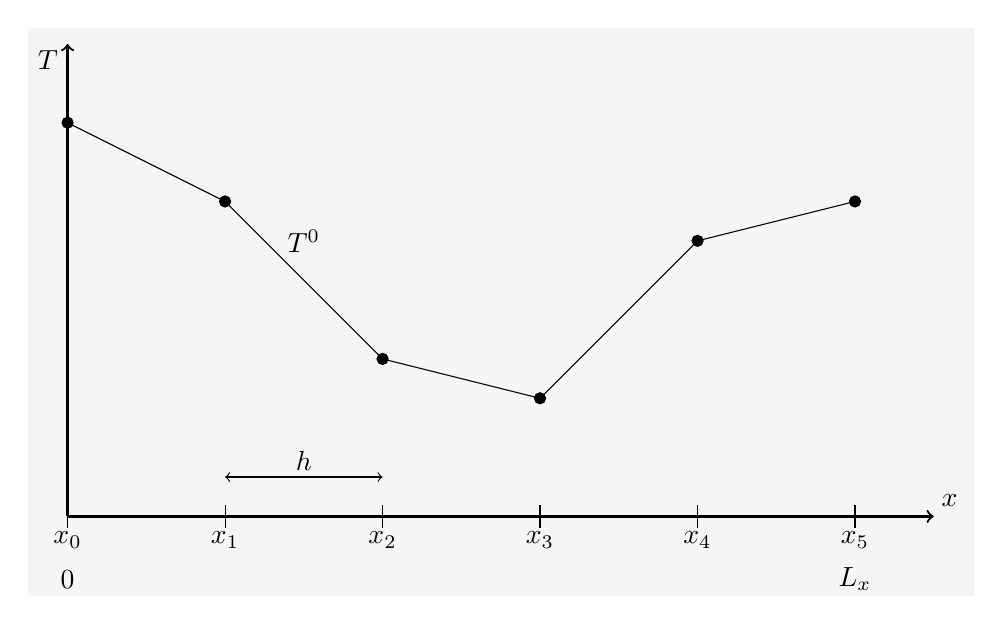
\begin{tikzpicture}
\draw[fill=gray!8,gray!8](0.5,0) rectangle (12.5,7.2);
%\draw[step=0.5cm,gray,very thin] (0,0) grid (13,7); %background grid

\draw[thick,->] (1,1) -- (12,1) ; 
\draw[thick,->] (1,1) -- (1,7) ; 


\node[] at (12.2,1.2) {$x$};
\node[] at (1,0.2) {$0$};
\node[] at (11,0.2) {$L_x$};
\node[] at (0.75,6.8) {$T$};

\draw[black,fill=black] (1,6)  circle (2pt);
\draw[black,fill=black] (3,5)  circle (2pt);
\draw[black,fill=black] (5,3)  circle (2pt);
\draw[black,fill=black] (7,2.5)  circle (2pt);
\draw[black,fill=black] (9,4.5)  circle (2pt);
\draw[black,fill=black] (11,5)  circle (2pt);

\draw[-] (1,6) -- (3,5) -- (5,3) -- (7,2.5) -- (9,4.5) -- (11,5); 
\node[] at (4,4.5) {$T^0$};

\draw[-] (1,0.85) -- (1,1.15) ; 
\draw[-] (3,0.85) -- (3,1.15) ; 
\draw[-] (5,0.85) -- (5,1.15) ; 
\draw[-] (7,0.85) -- (7,1.15) ; 
\draw[-] (9,0.85) -- (9,1.15) ; 
\draw[-] (11,0.85) -- (11,1.15) ; 
\node[] at (1,0.7) {$x_0$};
\node[] at (3,0.7) {$x_1$};
\node[] at (5,0.7) {$x_2$};
\node[] at (7,0.7) {$x_3$};
\node[] at (9,0.7) {$x_4$};
\node[] at (11,0.7) {$x_5$};
\draw[<->] (3,1.5) -- (5,1.5) ;  
\node[] at (4,1.7) {$h$};
\end{tikzpicture}


\end{center}

Then, we will be able to compute the new temperature of (for example) 
node 3 at time $t=1\cdot \delta t$ 
(i.e. $T_3^1$) with 
\begin{equation}
T_3^{1}=T_3^0 + \delta t \; \kappa \frac{T_{4}^0 - 2T_3^0 + T_{2}^0}{h^2}
\end{equation}
Note that $T_0$ and $T_5$ cannot be computed by means of the above equation, 
which is not a problem because both these values are actually the prescribed 
boundary conditions. 

\par\noindent\rule{\textwidth}{0.4pt}
\end{minipage}
\end{center}
%-/-/-/-/-/-/-/-/-/-/-/-/-/-/-/-/-/-/-/

\noindent The main drawback of the explicit approach is that stable solutions are
obtained {\it only} when
\begin{equation}
0 < \frac{2\kappa \delta t}{h^2} \leq1
\qquad
\text{or,}
\qquad
\delta t \leq \frac{h^2}{2 \kappa}
\end{equation}
If this condition is not satisfied, the solution becomes {\color{olive} unstable}, starts to
wildly oscillate and ultimately 'blows up'. We will observe this during the practicals. 

The stability condition means that the maximum time step needs to be smaller than the time it
takes for an anomaly to diffuse across the grid (nodal) spacing $h$.
The explicit solution is an example of a {\color{olive} conditionally stable method}
that only leads to well behaved solutions if a criterion like the one above is satisfied.

%-/-/-/-/-/-/-/-/-/-/-/-/-/-/-/-/-/-/-/-/-/
\begin{center}
\begin{minipage}[t]{0.77\textwidth}
\par\noindent\rule{\textwidth}{0.4pt}

\begin{center}

\includegraphics[width=0.8cm]{images/garftr} \\
{\color{orange}Exercise 2}
\end{center}

We are going to solve the 1D diffusion equation with the explicit method
for the following physical setup: The domain is $L_x=1$km long, 
it is maintained at a temperature $T=100\degree$C at $x=0$ and at a temperature
$T=200\degree$C at $x=L_x$. The initial temperature is $T(x,t=0)=123$
and $\kappa=10^{-6}$. 
Time stepping will be carried out until steady state is reached.

$\rightarrow$ 
\href{http://cedricthieulot.net/images/compgeo/Exercise_2_FDM.ipynb}
{\tt Exercise\_2\_FDM.ipynb}

\par\noindent\rule{\textwidth}{0.4pt}
\end{minipage}
\end{center}
%-/-/-/-/-/-/-/-/-/-/-/-/-/-/-/-/-/-/-/-/-/

\noindent An alternative approach is an {\bf implicit} finite difference scheme, where the spatial derivatives
of the Laplacian are evaluated (at least partially) at the new time step.
We then use the backward difference for the time derivative:
\begin{equation}
\frac{\partial T}{\partial t} = \frac{T_{i}^{n}-T_i^{n-1}}{\delta t} 
\end{equation}
so that
\begin{equation}
\frac{T_{i}^{n}-T_i^{n-1}}{\delta t} = \kappa \frac{T_{i+1}^n - 2T_i^n + T_{i-1}^n}{h^2}
\end{equation}
Note that this is often rewritten as follows in order to keep the unknwowns at time $n+1$:
\begin{equation}
\frac{T_{i}^{n+1}-T_i^{n}}{\delta t} = \kappa \frac{T_{i+1}^{n+1} - 2T_i^{n+1} + T_{i-1}^{n+1}}{h^2}
\end{equation}

It is a fully implicit scheme where the time derivative is taken backward.
Let us define the dimensionless parameter $s$ as follows:
\begin{equation}
s=\frac{\kappa \; \delta t}{h^2}
\end{equation}
The previous equation can be rearranged as follows:
\begin{equation}
\boxed{
-s \; T_{i+1}^{n+1} + (1+2s)\; T_{i}^{n+1} - s\; T_{i-1}^{n+1} = T_i^{n}
}
\end{equation}

\begin{center}
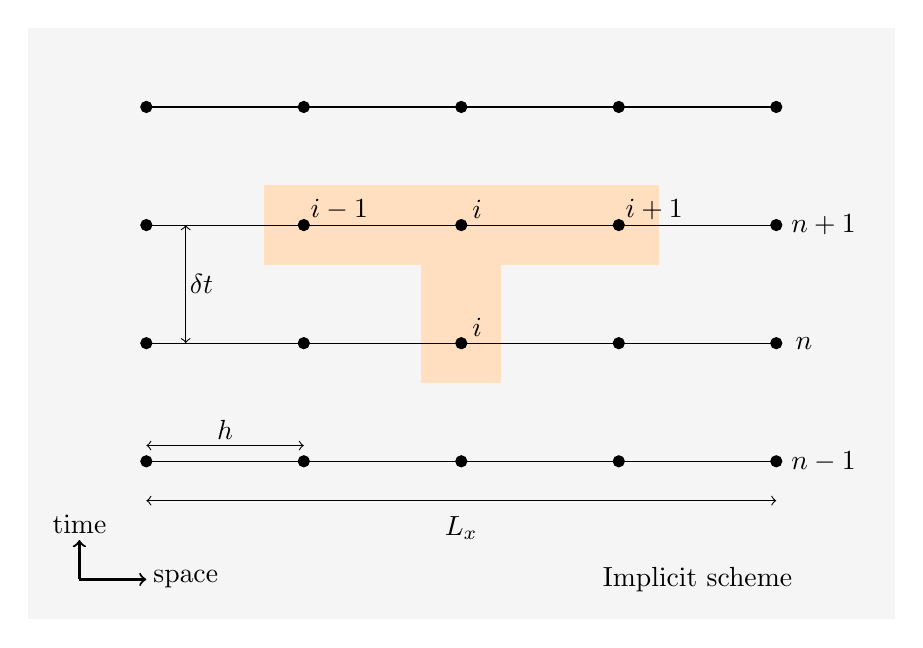
\begin{tikzpicture}
\draw[fill=gray!8,gray!8](-0.5,0) rectangle (10.5,7.5);

\draw[fill=orange,orange!25](2.5,4.5) rectangle (7.5,5.5);
\draw[fill=orange,orange!25](4.5,3) rectangle (5.5,4.5);
%\draw[step=0.5cm,gray,very thin] (0,0) grid (10.5,7.5); %background grid

\draw[black,fill=black] (1,2)  circle (2pt);
\draw[black,fill=black] (3,2)  circle (2pt);
\draw[black,fill=black] (5,2)  circle (2pt);
\draw[black,fill=black] (7,2)  circle (2pt);
\draw[black,fill=black] (9,2)  circle (2pt);

\draw[black,fill=black] (1,3.5)  circle (2pt);
\draw[black,fill=black] (3,3.5)  circle (2pt);
\draw[black,fill=black] (5,3.5)  circle (2pt);
\draw[black,fill=black] (7,3.5)  circle (2pt);
\draw[black,fill=black] (9,3.5)  circle (2pt);

\draw[black,fill=black] (1,5)  circle (2pt);
\draw[black,fill=black] (3,5)  circle (2pt);
\draw[black,fill=black] (5,5)  circle (2pt);
\draw[black,fill=black] (7,5)  circle (2pt);
\draw[black,fill=black] (9,5)  circle (2pt);

\draw[black,fill=black] (1,6.5)  circle (2pt);
\draw[black,fill=black] (3,6.5)  circle (2pt);
\draw[black,fill=black] (5,6.5)  circle (2pt);
\draw[black,fill=black] (7,6.5)  circle (2pt);
\draw[black,fill=black] (9,6.5)  circle (2pt);

\draw[-] (1,2) -- (9,2) ;
\draw[-] (1,3.5) -- (9,3.5) ;
\draw[-] (1,5) -- (9,5) ;
\draw[-] (1,6.5) -- (9,6.5) ;

\draw[<->] (1,2.2) -- (3,2.2) ;
\node[] at (2,2.4) {$h$};

\draw[<->] (1.5,3.5) -- (1.5,5) ;
\node[] at (1.7,4.25) {$\delta t$};

\draw[<->] (1,1.5) -- (9,1.5) ;
\node[] at (5,1.15) {$L_x$};

\draw[thick,->] (0.15,0.5) -- (1,0.5) ;
\draw[thick,->] (0.15,0.5) -- (0.15,1) ;
\node[] at (1.5,0.5) {space};
\node[] at (0.15,1.2) {time};

\node[] at (3.45,5.2) {$i-1$};
\node[] at (5.2,3.7) {$i$};
\node[] at (7.45,5.2) {$i+1$};
\node[] at (5.2,5.2) {$i$};

\node[] at (9.6,2) {$n-1$};
\node[] at (9.35,3.5) {$n$};
\node[] at (9.6,5) {$n+1$};

\node[] at (8,0.5) {Implicit scheme};
\end{tikzpicture}
                                                                                                                                                                                                                 



\end{center}



Note that in this case we no longer have an explicit relationship for 
$T^{n+1}_{i-1}$, $T^{n+1}_i$ and $T^{n+1}_{i+1}$.
Instead, we have to solve a {\color{olive}linear system of equations}, which is discussed further below.

The main advantage of implicit methods is that there are no restrictions on the time step,
the fully implicit scheme is {\bf unconditionally stable}.
This does not mean that it is accurate. 
Taking large time steps may result in an inaccurate solution for features with
small spatial scales!

For any application, it is therefore always a good idea to check the 
results by decreasing the time step
until the solution does not change anymore (this is called a {\color{olive}convergence check}), and 
to ensure the
method can deal with small and large scale features robustly at the same time.


%-/-/-/-/-/-/-/-/-/-/-/-/-/-/-/-/-/-/-
\begin{center}
\begin{minipage}[t]{0.77\textwidth}
\par\noindent\rule{\textwidth}{0.4pt}
{\color{blue} Example}: 
Once again let us look at things with a very concrete approach. Let us discretise the 
domain of length $L_x$ with 6 cells, i.e. $i=0,\dots 6$ ($nnx=7$).
We also prescribe the following boundary conditions (remember it is a 2nd order derivative in space, 
so we need two of them): $T(x=0)=T_0=0$ and $T(x=L_x)=T_6=100$ (we assume that they 
do not change with time for simplicity). Finally we assume that we 
know $T_i^0$ for all $i$ and we wish to compute $T_i^1$.

We then have:
\begin{eqnarray}
T_0^1 &=& 0 \nn\\
-s T_{2}^{1} + (1+2s) T_{1}^{1} - s T_{0}^{1} &=& T_1^{0} \nn\\
-s T_{3}^{1} + (1+2s) T_{2}^{1} - s T_{1}^{1} &=& T_2^{0} \nn\\
-s T_{4}^{1} + (1+2s) T_{3}^{1} - s T_{2}^{1} &=& T_3^{0} \nn\\
-s T_{5}^{1} + (1+2s) T_{4}^{1} - s T_{3}^{1} &=& T_4^{0} \nn\\
-s T_{6}^{1} + (1+2s) T_{5}^{1} - s T_{4}^{1} &=& T_5^{0} \nn\\
T_6^1 &=& 100
\end{eqnarray}
or, 
\begin{equation}
\underbrace{
\left(
\begin{array}{ccccccc}
1 & 0 & 0 & 0 & 0 & 0 & 0  \\
-s & 1+2s & -s & 0 & 0 & 0 & 0 \\
0 & -s & 1+2s & -s & 0 & 0 & 0 \\
0 & 0 & -s & 1+2s & -s & 0 & 0 \\
0 & 0 & 0 & -s & 1+2s & -s & 0 \\
0 & 0 & 0 & 0 & -s & 1+2s & -s \\
0 & 0 & 0 & 0 & 0 & 0 & 1
\end{array}
\right)
}_{\bm A}
\cdot
\underbrace{
\left(
\begin{array}{ccccccc}
T_0^1 \\ T_1^1 \\ T_2^1 \\ T_3^1 \\ T_4^1 \\ T_5^1 \\ T_6^1  
\end{array}
\right)
}_{\vec{T}}
=
\underbrace{
\left(
\begin{array}{ccccccc}
0 \\ T_1^0\\ T_2^0\\ T_3^0\\ T_4^0\\ T_5^0 \\ 100
\end{array}
\right)
}_{\vec{b}} \nn
\end{equation}

As opposed to the explicit approach we must solve a linear system which size is given 
by the total number of nodes/points $nnx$ in order to compute a new temperature field.

\par\noindent\rule{\textwidth}{0.4pt}
\end{minipage}
\end{center}
%-/-/-/-/-/-/-/-/-/-/-/-/-/-/-/-/-/-/-

\noindent In summary, an implicit method requires us to solve ${\bm A}\cdot\vec{T} = \vec{b}$ with
\begin{itemize}
\item ${\bm A}$ is a $nnx \times nnx$  {\color{olive}sparse} matrix (i.e. mostly empty),
\item ${\vec b}$ is a known vector of size $nnx$ (often called the 'right-hand side', or {\color{olive} rhs})
\item ${\vec T}$ the vector of unknowns.
\end{itemize}

%..................................
\paragraph{A word about solvers}
There are two main approaches to solving such a linear system: one can use a {\color{olive} direct}
approach or an {\color{olive} iterative} approach. 
In a nutshell, a direct solver will 'manipulate' the matrix lines and columns 
so as to arrive at the solution. A simple example of such an approach is the 
technique of elimination of variables:

\begin{center}
\begin{minipage}[t]{0.77\textwidth}
\par\noindent\rule{\textwidth}{0.4pt}
{\color{blue} Example}:
Consider the following system:
\begin{equation}
\left(
\begin{array}{ccc}
1 & 3 & -2 \\
3 & 5 & 6 \\
2 & 4 & 3
\end{array}
\right)
\cdot
\left(
\begin{array}{c}
x \\ y \\ z
\end{array}
\right)
=
\left(
\begin{array}{c}
5 \\ 7 \\ 8
\end{array}
\right)
\end{equation}
which is of course equivalent to
\begin{eqnarray}
x+3y-2z &=& 5 \nn\\
3x+5y+6z &=& 7 \nn\\
2x+4y+3z &=& 8 
\end{eqnarray}
Solving the first equation for $x$ gives $x = 5 + 2z - 3y$, 
and plugging this into the second and third equation yields
(or take the second line of the matrix and remove 3 times the 
first line from it, etc ...)
\begin{equation}
\left(
\begin{array}{ccc}
1 & 3 & -2 \\
0 & -4 & 12 \\
0 & -2 & 7
\end{array}
\right)
\cdot
\left(
\begin{array}{c}
x \\ y \\ z
\end{array}
\right)
=
\left(
\begin{array}{c}
5 \\ -8 \\ -2 
\end{array}
\right)
\end{equation}
Solving the second line for $y$ yields $y = 2 + 3z$, 
and plugging this into the second equation yields $z = 2$. We now have: 
\begin{equation}
\left(
\begin{array}{ccc}
1 & 3 & -2 \\
0 & -4 & 12 \\
0 & 0 & 2
\end{array}
\right)
\cdot
\left(
\begin{array}{c}
x \\ y \\ z
\end{array}
\right)
=
\left(
\begin{array}{c}
5 \\ -8 \\ 4
\end{array}
\right)
\end{equation}
Substituting $z = 2$ into the second equation gives $y = 8$, 
and substituting $z = 2$ and $y = 8$ into the first equation yields $x = -15$. 
Therefore, the solution set is the single point $(x, y, z) = (-15, 8, 2)$.

{\tiny Taken from \url{https://en.wikipedia.org/wiki/System_of_linear_equations}} 
\par\noindent\rule{\textwidth}{0.4pt}
\end{minipage}
\end{center}

This example is of course very naive and direct solvers often come in 
the form of very large numerical libraries which have been highly optimised to take advantage of the 
sparsity of the matrix in order to arrive at the solution in the lowest 
number of operations possible. 
In reality techniques such as LU decomposition or Cholesky decomposition are used. 
\index{general}{LU decomposition}
\index{general}{Cholesky decomposition}

Iterative solvers on the other hand compute the solution of the system 
by first postulating an initial guess for the solution and then by 
improving this guess iteratively until the {\color{olive} termination criterion}
is met. There are two classes of iteratives methods in this context: 
{\color{olive} stationary iterative methods} (e.g. Jacobi, Gauss-Seidel, SSOR) and 
{\color{olive} Krylov subspace methods} (e.g. CG, GMRES, BiCG).
At this stage things get real complicated and the details of iterative solvers 
are vastly out of the scope of this 
course\footnote{\url{https://en.wikipedia.org/wiki/Iterative_method}} \cite{saad}.     
\index{general}{BiCG solver}
\index{general}{Jacobi solver}
\index{general}{Gauss-Seidel solver}
\index{general}{GMRES solver}
\index{general}{CG solver}
\index{general}{SSOR solver}


%-/-/-/-/-/-/-/-/-/-/-/-/-/-/-/-/-/-/-/-/-/
\begin{center}
\begin{minipage}[t]{0.77\textwidth}
\par\noindent\rule{\textwidth}{0.4pt}
{\color{blue} Example}: the stationary Jacobi method. 
The matrix ${\bm A}$ is decomposed as follows:
\begin{equation}
{\bm A} = {\bm D} + {\bm L} + {\bm U} 
\end{equation}
where ${\bm D}$ is the diagonal of the matrix ${\bm A}$, ${\bm L}$ is the 
strict lower triangular part of ${\bm A}$ and 
${\bm U}$ is the strict upper triangular part of ${\bm A}$.
The iterative method is defined by:
\begin{equation}
{\bm D} \cdot \vec{T}^{{\color{Fuchsia}k+1}} = -({\bm L} + {\bm U}) \cdot \vec{T}^{\color{Fuchsia}k} 
+ \vec{b}
\qquad k=0,1,\dots
\end{equation}
where $\vec{T}^{\color{Fuchsia}0}$ is the initial guess (often taken to be zero).
Note that the superscript denotes the iteration number and has nothing to 
do with the time step.
This method is trivial to implement since the linear system on the 
left side of the equal sign involves a diagonal matrix.
This can also be written 
\begin{equation}
T_i^{{\color{Fuchsia} k+1}} = \frac{1}{A_{ii}} \left(b_i - 
\sum_{j\neq i} A_{ij} T_j^{{\color{Fuchsia}k}} \right)
\qquad
i=1,2,...nnx
\end{equation}
Looking at the previous example, we have 
\begin{equation}
{\bm D}=
\left(
\begin{array}{ccc}
1 & 0 & 0 \\
0 & 5 & 0 \\
0 & 0 & 3
\end{array}
\right)
\qquad
\text{and}
\qquad
{\bm L}+{\bm U}= 
\left(
\begin{array}{ccc}
0 & 3 & -2 \\
3 & 0 & 6 \\
2 & 4 & 0
\end{array}
\right)
\end{equation}
We then start with the guess $\vec{T}^{\color{Fuchsia}0}=\vec{0}$, so that for ${\color{Fuchsia}k}=1$:
\begin{equation}
\vec{T}^{\color{Fuchsia}1} = {\bm D}^{-1}\cdot \vec{b} = 
\left(
\begin{array}{ccc}
1 & 0 & 0 \\
0 & 1/5 & 0 \\
0 & 0 & 1/3
\end{array}
\right)
\cdot 
\left(
\begin{array}{c}
5 \\ 7 \\ 8
\end{array}
\right)
=
\left(
\begin{array}{c}
5 \\ 7/5 \\ 8/3
\end{array}
\right)
\end{equation}
and then we obtain $\vec{T}^{\color{Fuchsia}2}$ by solving 
\begin{eqnarray}
\vec{T}^{\color{Fuchsia}2} 
&=& {\bm D}^{-1} \cdot \left[-({\bm L} + {\bm U}) 
\cdot \vec{T}^{\color{Fuchsia}1} + \vec{b} \right] \nn\\
&=&
\left(
\begin{array}{ccc}
1 & 0 & 0 \\
0 & 1/5 & 0 \\
0 & 0 & 1/3
\end{array}
\right)
\cdot 
\left[
-
\left(
\begin{array}{ccc}
0 & 3 & -2 \\
3 & 0 & 6 \\
2 & 4 & 0
\end{array}
\right)
\cdot
\left(
\begin{array}{c}
5 \\ 7/5 \\ 8/3
\end{array}
\right)
+
\left(
\begin{array}{c}
5 \\ 7 \\ 8
\end{array}
\right)
\right] \nn\\
&=&
\dots  
\end{eqnarray}
We keep iterating until two consecutively obtained 
temperature vectors are nearly identical, or, 
\begin{equation}
\| \vec{T}^{\color{Fuchsia}k+1}-\vec{T}^{\color{Fuchsia}k} \| < \epsilon
\end{equation}
where $\epsilon$ is a carefully chosen small enough number. 

A sufficient (but not necessary) condition for the method to converge is that 
the matrix ${\bm A}$ is strictly or irreducibly diagonally dominant. 
Strict row diagonal dominance means that for each row, the absolute value of 
the diagonal term is greater than the sum of absolute values of other 
terms $|a_{ii}|>\sum_{j\neq i} |a_{ij}| $.
Also, this algorithm will fail if one or more diagonal terms of ${\bm A}$ is nul.

\par\noindent\rule{\textwidth}{0.4pt}
\end{minipage}
\end{center}
%-/-/-/-/-/-/-/-/-/-/-/-/-/-/-/-/-/-/-/-/-/


%-/-/-/-/-/-/-/-/-/-/-/-/-/-/-/-/-/-/-/
\begin{center}
\begin{minipage}[t]{0.77\textwidth}
\par\noindent\rule{\textwidth}{0.4pt}

\begin{center}

\includegraphics[width=0.8cm]{images/garftr} \\
{\color{orange}Exercise 3}
\end{center}

Implement the above example from scratch in a new notebook.
What do you observe ? why does it explode? 
Multiply all diagonal values by 10 and re-run it. 
What do you observe now? 


Bonus: implement the Gauss-Seidel method\footnote{
\url{https://en.wikipedia.org/wiki/Iterative_method}}. 
Which of the two methods converges the fastest?
\par\noindent\rule{\textwidth}{0.4pt}
\end{minipage}
\end{center}
%-/-/-/-/-/-/-/-/-/-/-/-/-/-/-/-/-/-/-/


\noindent
Finally, looking at
\begin{equation}
-s\;  T_{i+1}^{n+1} + (1+2s)\;  T_{i}^{n+1} - s\;  T_{i-1}^{n+1} = T_i^{n}
\end{equation}
and dividing by $-s$ and letting $\delta t \rightarrow \infty$, we obtain:
\begin{equation}
T_{i+1}^{n+1} -2 T_{i}^{n+1} + T_{i-1}^{n+1} = 0
\end{equation}
which is a central difference approximation of the steady state solution
\begin{equation}
\frac{\partial^2 T }{\partial x^2}=0
\end{equation}
Therefore, the fully implicit scheme will always yield the right equilibrium solution 
but may not capture small scale, transient features.


%-/-/-/-/-/-/-/-/-/-/-/-/-/-/-/-/-/-/-/
\begin{center}
\begin{minipage}[t]{0.77\textwidth}
\par\noindent\rule{\textwidth}{0.4pt}

\begin{center}

\includegraphics[width=0.8cm]{images/garftr} \\
{\color{orange}Exercise 4}
\end{center}

This is exactly the same exercise as Exercise 2 but we 
are going to solve the 1D diffusion equation with the implicit method
this time. First use a solver from scipy to solve the system, then 
implement your own Jacobi solver. 

In your notebook use an if statement which allows to choose between 
explicit and implicit, and another if statement which allows to choose 
between scipy solver and iterative solver. 

Bonus: implement the SSOR method\footnote{
\url{https://en.wikipedia.org/wiki/Iterative_method}}
and compare Jacobi, Gauss-Seidel and SSOR.

\par\noindent\rule{\textwidth}{0.4pt}
\end{minipage}
\end{center}
%-/-/-/-/-/-/-/-/-/-/-/-/-/-/-/-/-/-/-/


\paragraph{Crank-Nicolson scheme} \index{general}{Crank-Nicolson}
It turns out that this fully implicit method is second order accurate in space but 
only first order accurate in time,
i.e. the error goes as ${\cal O}(h^2,\delta t)$.   

It is possible to write down a scheme which is second order accurate both in time and in space
(i.e. ${\cal O}(h^2, \delta t^2))$, e.g. the {\color{olive}Crank-Nicolson}
\footnote{
The method was developed by John Crank and Phyllis Nicolson 
in the mid 20th century. \url{https://en.wikipedia.org/wiki/Crank-Nicolson_method}
}
scheme which is unconditionally stable. 

The Crank-Nicolson method is the time analog of central spatial differences and is given by
\begin{equation}
\frac{T_{i}^{n+1}-T_i^n}{\delta t} 
= \kappa  \frac{1}{2} \left[
\underbrace{\frac{T_{i+1}^{n} - 2T_i^{n} + T_{i-1}^{n}}{h^2}}_{\text{at time } n}
+
\underbrace{\frac{T_{i+1}^{n+1} - 2T_i^{n+1} + T_{i-1}^{n+1}}{h^2}}_{\text{at time } n+1}
\right]
\end{equation}
We define $s=\kappa \delta t/ 2h^2$ so that the equation above can be rearranged as follows :
\begin{equation}
\boxed{
-s\; T_{i+1}^{n+1} + (1+2s)\;  T_{i}^{n+1} 
-s\;  T_{i-1}^{n+1} = 
s\; T_{i+1}^{n} + (1-2s)\; T_{i}^{n} + s\; T_{i-1}^{n} 
}
\end{equation}

Any partially implicit method is more complicated to compute as we need to infer the future solution 
at time $n+1$ by solution (inversion) of a system of linear equations based on the known solution at time $n$. 

\begin{center}

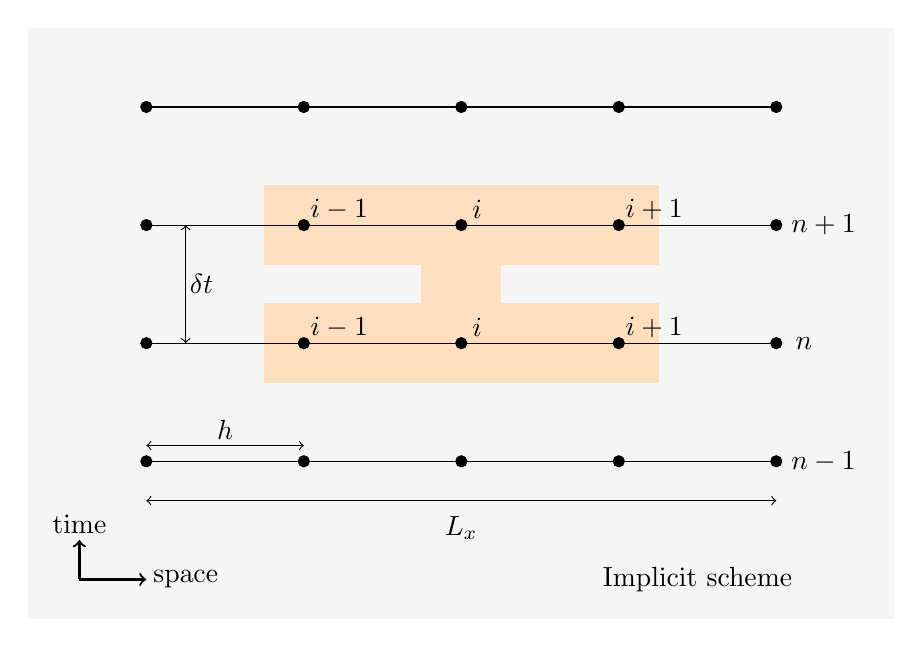
\begin{tikzpicture}
\draw[fill=gray!8,gray!8](-0.5,0) rectangle (10.5,7.5);


\draw[fill=orange,orange!25](2.5,4.5) rectangle (7.5,5.5);
\draw[fill=orange,orange!25](4.5,3) rectangle (5.5,4.5);
\draw[fill=orange,orange!25](2.5,3) rectangle (7.5,4);

%\draw[step=0.5cm,gray,very thin] (0,0) grid (10.5,7.5); %background grid

\draw[black,fill=black] (1,2)  circle (2pt);
\draw[black,fill=black] (3,2)  circle (2pt);
\draw[black,fill=black] (5,2)  circle (2pt);
\draw[black,fill=black] (7,2)  circle (2pt);
\draw[black,fill=black] (9,2)  circle (2pt);

\draw[black,fill=black] (1,3.5)  circle (2pt);
\draw[black,fill=black] (3,3.5)  circle (2pt);
\draw[black,fill=black] (5,3.5)  circle (2pt);
\draw[black,fill=black] (7,3.5)  circle (2pt);
\draw[black,fill=black] (9,3.5)  circle (2pt);

\draw[black,fill=black] (1,5)  circle (2pt);
\draw[black,fill=black] (3,5)  circle (2pt);
\draw[black,fill=black] (5,5)  circle (2pt);
\draw[black,fill=black] (7,5)  circle (2pt);
\draw[black,fill=black] (9,5)  circle (2pt);

\draw[black,fill=black] (1,6.5)  circle (2pt);
\draw[black,fill=black] (3,6.5)  circle (2pt);
\draw[black,fill=black] (5,6.5)  circle (2pt);
\draw[black,fill=black] (7,6.5)  circle (2pt);
\draw[black,fill=black] (9,6.5)  circle (2pt);

\draw[-] (1,2) -- (9,2) ;
\draw[-] (1,3.5) -- (9,3.5) ;
\draw[-] (1,5) -- (9,5) ;
\draw[-] (1,6.5) -- (9,6.5) ;

\draw[<->] (1,2.2) -- (3,2.2) ;
\node[] at (2,2.4) {$h$};

\draw[<->] (1.5,3.5) -- (1.5,5) ;
\node[] at (1.7,4.25) {$\delta t$};

\draw[<->] (1,1.5) -- (9,1.5) ;
\node[] at (5,1.15) {$L_x$};

\draw[thick,->] (0.15,0.5) -- (1,0.5) ;
\draw[thick,->] (0.15,0.5) -- (0.15,1) ;
\node[] at (1.5,0.5) {space};
\node[] at (0.15,1.2) {time};

\node[] at (3.45,3.7) {$i-1$};
\node[] at (3.45,5.2) {$i-1$};
\node[] at (5.2,3.7) {$i$};
\node[] at (7.45,5.2) {$i+1$};
\node[] at (7.45,3.7) {$i+1$};
\node[] at (5.2,5.2) {$i$};

\node[] at (9.6,2) {$n-1$};
\node[] at (9.35,3.5) {$n$};
\node[] at (9.6,5) {$n+1$};

\node[] at (8,0.5) {Implicit scheme};
\end{tikzpicture}
                                                                                                                                                                                                                 




\end{center}

%-/-/-/-/-/-/-/-/-/-/-/-/-/-/-/-/-/-/
\begin{center}
\begin{minipage}[t]{0.77\textwidth}
\par\noindent\rule{\textwidth}{0.4pt}

\begin{center}

\includegraphics[width=0.8cm]{images/garftr} \\
{\color{orange}Exercise 5}
\end{center}

Modify the code of exercise 4 to implement the Crank-Nicolson method.

\par\noindent\rule{\textwidth}{0.4pt}
\end{minipage}
\end{center}
%-/-/-/-/-/-/-/-/-/-/-/-/-/-/-/-/-/-/





